\documentclass[10pt]{beamer}

% --- Configuración de Tema ---
\usetheme{Madrid}
\usecolortheme{default}
\setbeamertemplate{navigqation symbols}{} % Quitar iconos de navegación

% --- Paquetes ---
\usepackage[spanish]{babel}
\usepackage[utf8]{inputenc}
\usepackage{graphicx}
	\graphicspath{{../img}}
\usepackage{amsmath}
\usepackage{siunitx}
\usepackage{listings}
\usepackage{booktabs}

% Configuración de listings para código C
\lstset{
    language=C,
    basicstyle=\ttfamily\tiny,
    keywordstyle=\color{blue},
    commentstyle=\color{green!60!black},
    stringstyle=\color{orange},
    breaklines=true,
    frame=single
}

% --- Información del Proyecto ---
\title[Sensor de Colores]{Desarrollo de un Sensor de Colores por Reflexión}
\subtitle{Técnicas Digitales III}
\author[Beck, Perez]{Federico Beck \and Mariano Perez}
\institute[UTN FRSF]{
    Departamento de Ingeniería Electrónica\\
    Facultad Regional San Francisco --- UTN
}
\date{8 de Abril, 2026}

% Logo en la esquina (opcional)
\titlegraphic{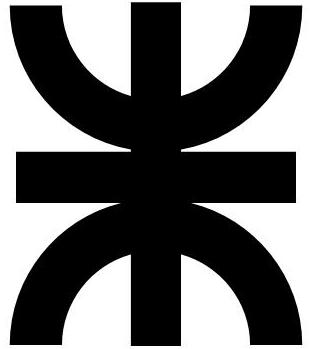
\includegraphics[height=1cm]{UTN_logo.jpg}}

\begin{document}

% --- Diapositiva de Título ---
\begin{frame}
    \titlepage{}
\end{frame}

% --- Índice ---
\begin{frame}{Contenidos}
    \tableofcontents
\end{frame}

% --- Introducción ---
\section{Introducción}
\begin{frame}{Introducción y Motivación}
    \begin{columns}
        \begin{column}{0.5\textwidth}
            \begin{itemize}
                \item \textbf{Objetivo:} Dispositivo de bajo costo para determinación de color.
                \item \textbf{Principio:} Reflexión de luz roja, verde y azul sobre una superficie.
                \item \textbf{Sensor:} Resistencia dependiente de la luz (LDR).
            \end{itemize}
        \end{column}
        \begin{column}{0.5\textwidth}
            \centering
            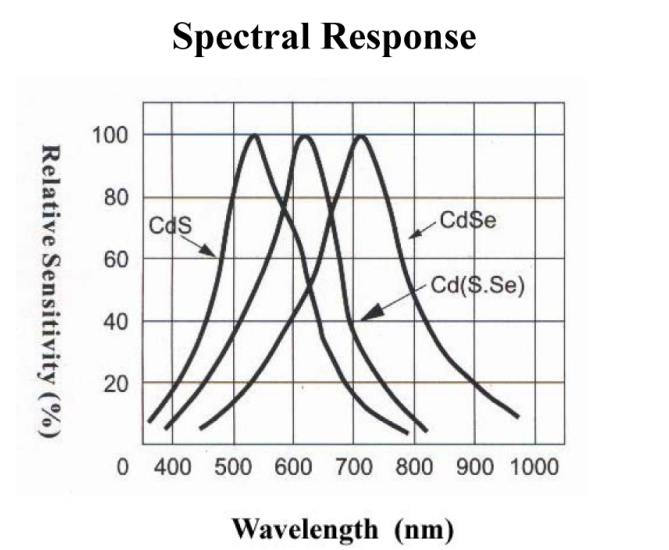
\includegraphics[width=\textwidth]{LDR_spectral_response.png}
            % cambiar x diagrama general
        \end{column}
    \end{columns}
\end{frame}

\begin{frame}{Opciones Comerciales}
    \begin{itemize}
        \item Utiliza luz blanca, filtros, y un fotodiodo.
    \end{itemize}

    \begin{figure}
        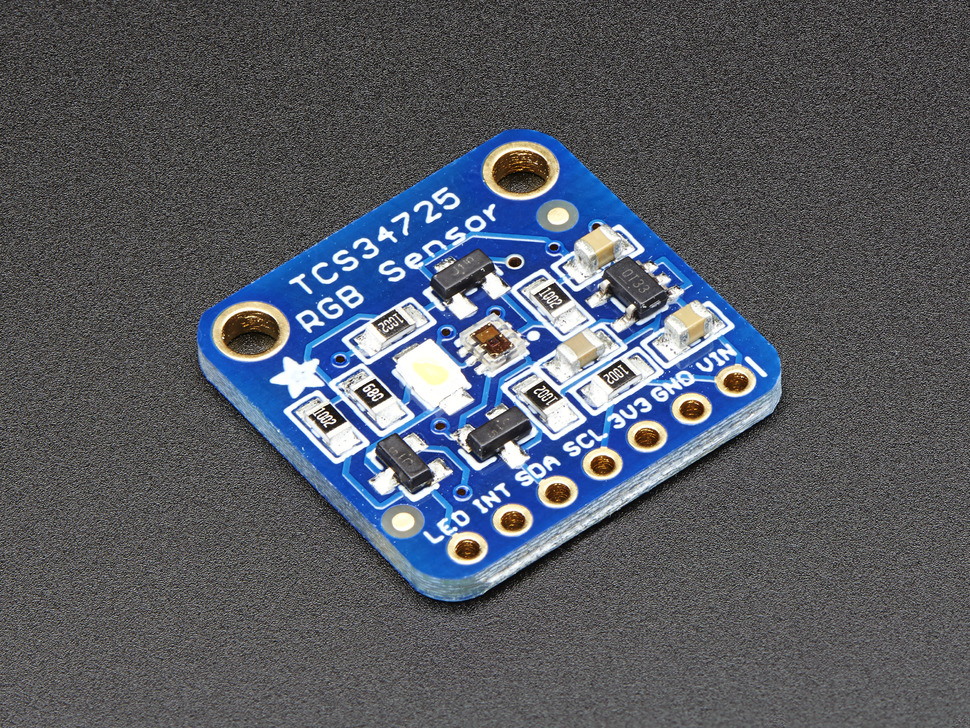
\includegraphics[width=0.5\textwidth]{beamer/tcs_34725_color_sensor.png}
        \caption{Sensor de color Adafruit TCS34725.}
    \end{figure}
\end{frame}

% --- Hardware y Diseño ---
\section{Hardware y Diseño}
\begin{frame}{Diseño Físico y Carcasa}
    \begin{itemize}
        \item Aislamiento de luz ambiente para evitar distorsión en mediciones.
        \item Compartimientos separados para LEDs, LDR y conexiones.
    \end{itemize}
    \centering
    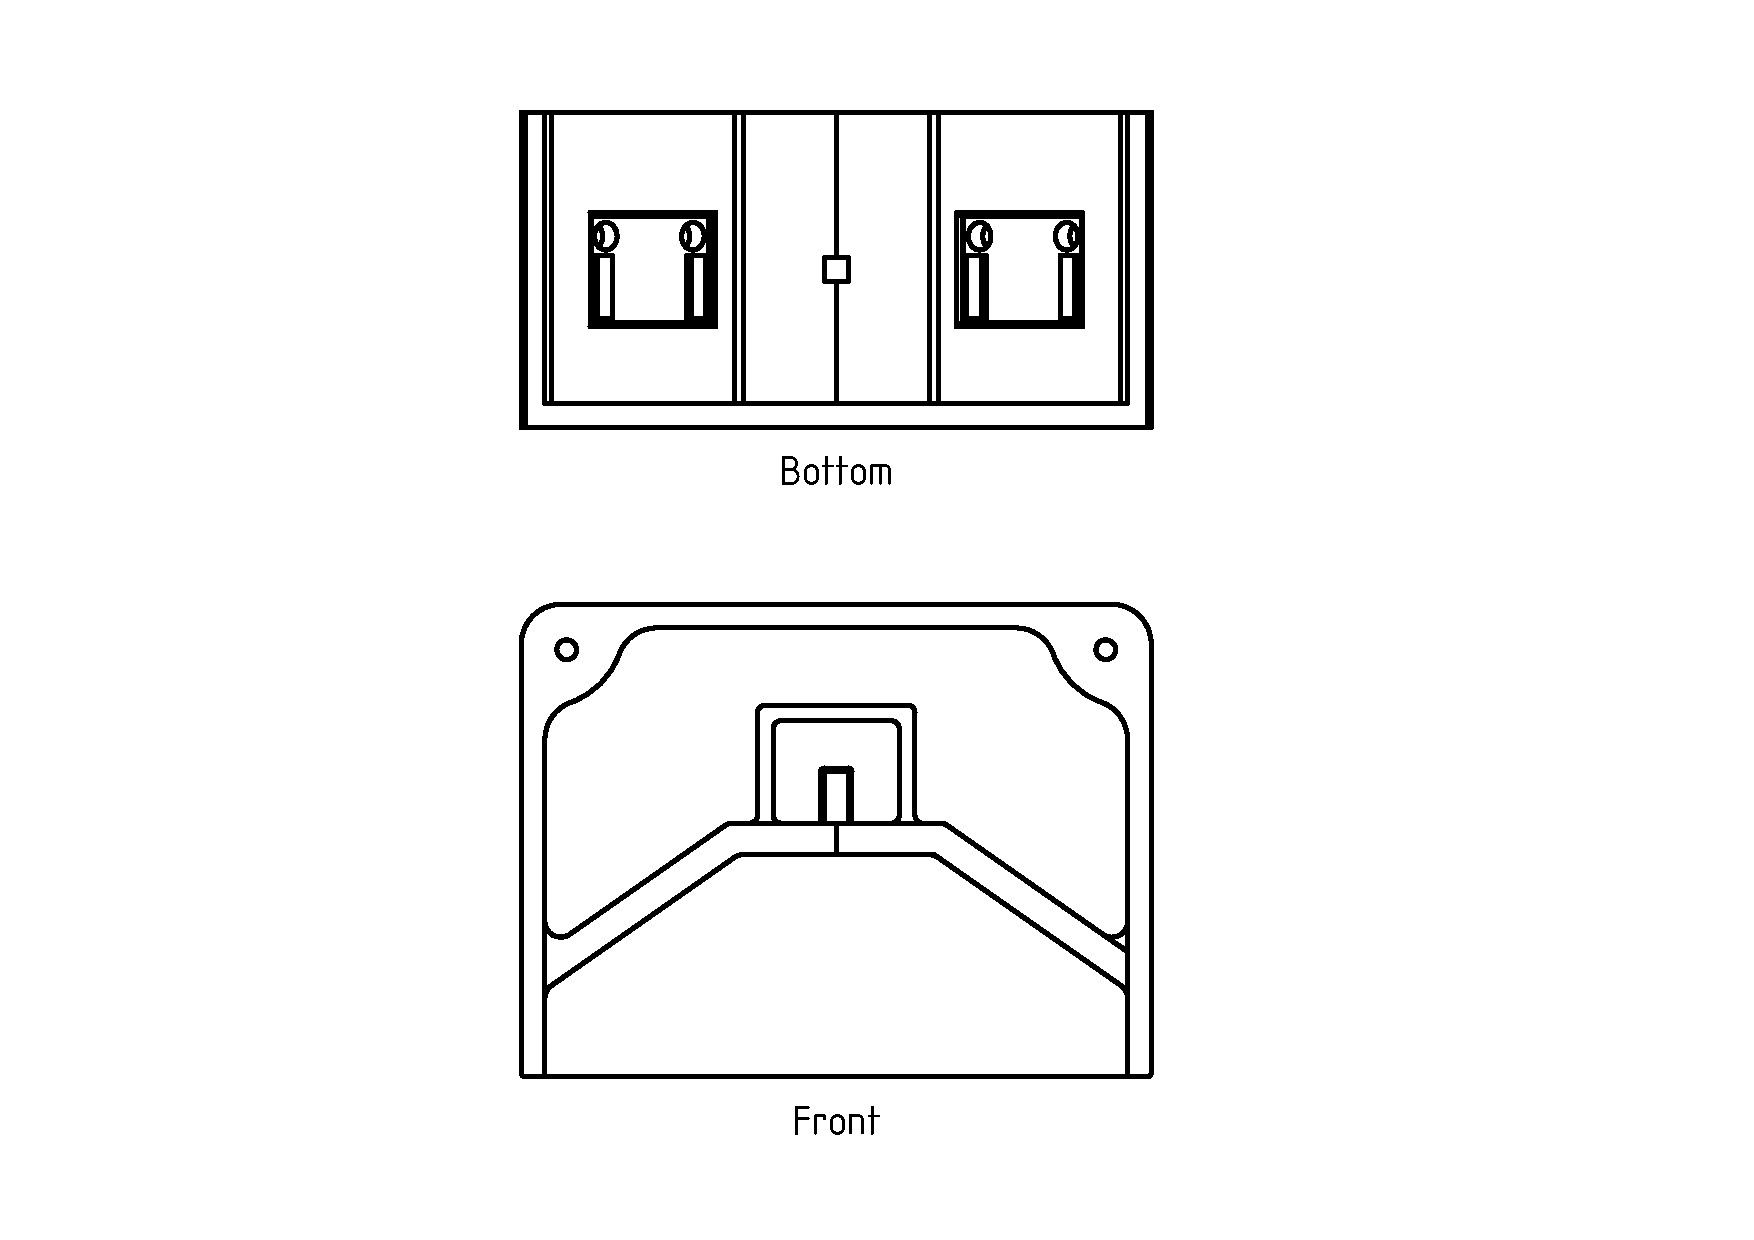
\includegraphics[width=0.7\textwidth]{vistas_carcasa.pdf}
    % \captionof{figure}{Vistas de la carcasa diseñada.}
\end{frame}

\begin{frame}{Componentes Electrónicos: Transductor}
    \begin{columns}
        \begin{column}{0.5\textwidth}
        \end{column}
        \begin{column}{0.5\textwidth}
            \begin{figure}
                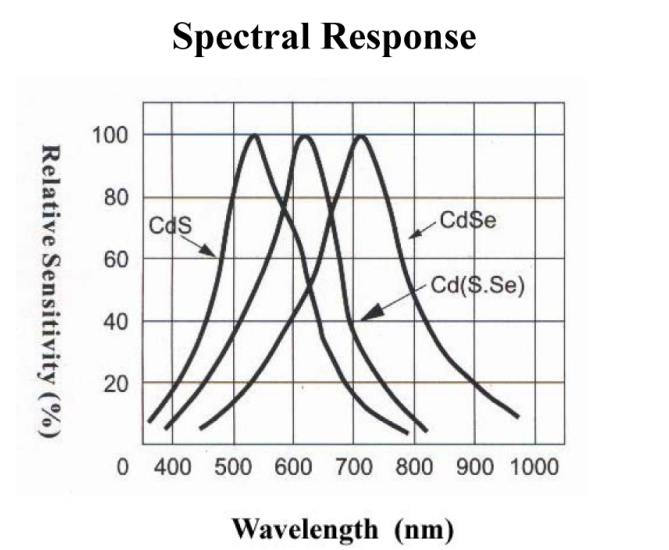
\includegraphics[width=\textwidth]{LDR_spectral_response.png}
                \caption{Respuesta espectral de distintos tipos de LDR.}
            \end{figure}
        \end{column}
    \end{columns}
\end{frame}

\begin{frame}{Componentes Electrónicos}
    \begin{columns}
        \begin{column}{0.5\textwidth}
            \textbf{Unidad de Control:}
            \begin{itemize}
                \item Raspberry Pi Pico (RP2040).
                \item DMA para muestreo de ADC.
            \end{itemize}
            \textbf{Iluminantes:}
            \begin{itemize}
                \item LEDs WS2812 (RGB).
                \item Control preciso mediante \textbf{PIO} (I/O programable).
            \end{itemize}
        \end{column}
        \begin{column}{0.5\textwidth}
            \centering
            %             \rule{4cm}{3cm} % Placeholder para foto del hardware real
        \end{column}
    \end{columns}
    \begin{block}{Ventajas del RP2040}
        Doble núcleo ARM Cortex-M0+ y stack USB integrado.
    \end{block}
\end{frame}

% --- Circuito de Acondicionamiento ---
\section{Circuito de Acondicionamiento}
\begin{frame}{Acondicionamiento de Señal}
    \centering
    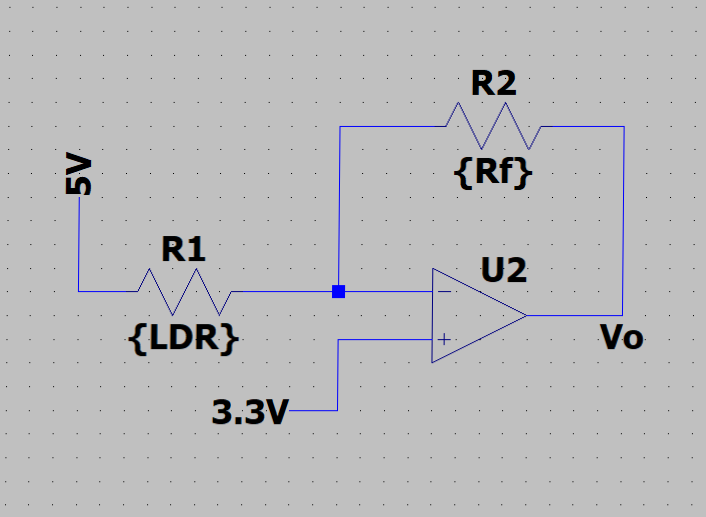
\includegraphics[width=0.55\textwidth]{circ_acond.png}
    % \captionof{figure}{Esquemático: Amplificador inversor con offset.}
    
    \begin{equation*}
        V_o = V_{+} + (V_{+} - V_{s}) \frac{R_f}{R_{LDR}} \text{ }
    \end{equation*}

    \begin{itemize}
        \item \textbf{Control de Ganancia:} Switch CD4066 para alternar $R_f$ (\qtylist{1;10;100}{\kohm}).
        \item Evita la saturación ante el amplio rango del LDR (\qtyrange{1}{1000}{\kohm}).
    \end{itemize}
\end{frame}

\begin{frame}{Respuesta del Circuito}
    \begin{figure}[htbp]
        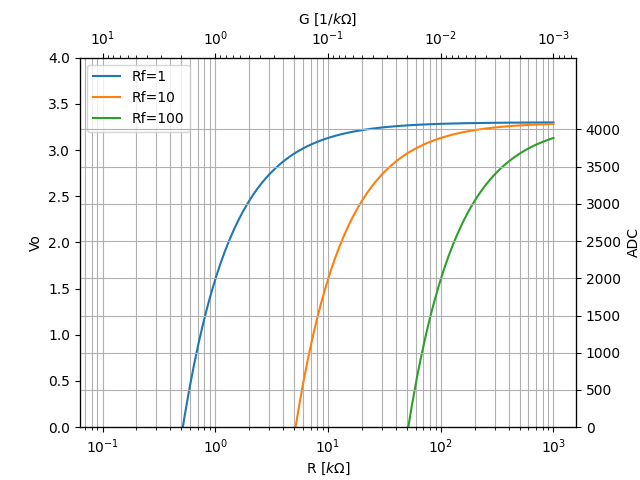
\includegraphics[width=0.7\textwidth]{circuit_response.png}
        \caption{Tensión de salida vs Resistencia del LDR para distintas $R_f$.}
    \end{figure}
\end{frame}

% --- Caracterización ---
\section{Caracterización del LDR}
\begin{frame}{Modelo Matemático y Calibración}
    \begin{columns}
        \begin{column}{0.5\textwidth}
            La respuesta del LDR no es lineal:
            \begin{equation*}
                G = K_a c^{\gamma} \text{ }
            \end{equation*}
            \begin{itemize}
                \item $G$: Conductancia.
                \item $c$: Intensidad del LED.
                \item $K_a, \gamma$: Parámetros empíricos.
            \end{itemize}
        \end{column}
        \begin{column}{0.5\textwidth}
            \centering
            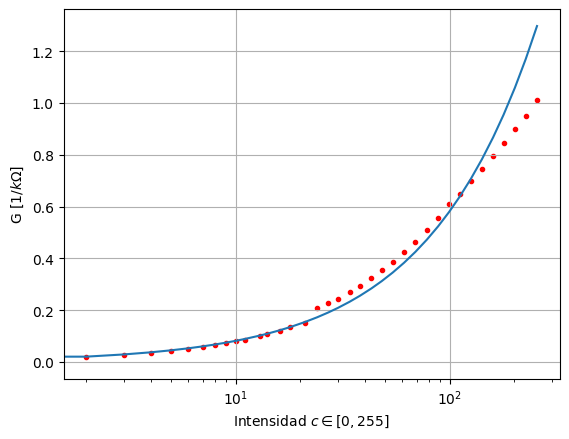
\includegraphics[width=\textwidth]{conductancia_intensidad_LSQ.png}
            % \captionof{figure}{Ajuste por Mínimos Cuadrados.}
        \end{column}
    \end{columns}
\end{frame}

\begin{frame}{Proceso de Medicion}

\end{frame}

% --- Firmware ---
\section{Firmware}
\begin{frame}{Arquitectura del Firmware (FreeRTOS)}
    \begin{itemize}
        \item Implementación en C usando \textbf{Pico-SDK} y \textbf{TinyUSB}.
        \item División de tareas para manejar la asincronía del USB.
    \end{itemize}
    \begin{center}
        \begin{tabular}{ll}
            \toprule
            \textbf{Tarea} & \textbf{Función} \\
            \midrule
            \texttt{usb\_task()} & Maneja el stack USB y comunicación con Host. \\
            \texttt{worker\_task()} & Ejecuta comandos (muestreo, LEDs). \\
            \bottomrule
        \end{tabular}
    \end{center}
\end{frame}

\begin{frame}[fragile]{Código: Gestión de Comunicación USB}
\begin{lstlisting}[caption={Estructura de la tarea usb\_task() }]
void usb_task(void *arg) {
    while (1) {
        tud_task(); // Ejecuta el stack USB
        if (!msg_in_buffer) {
            size_t n = xMessageBufferReceive(tx_msg_buffer, ...);
        }
        if (msg_in_buffer) {
            tud_cdc_write(...);
        }
    }
}
\end{lstlisting}
\end{frame}

% --- Conclusión ---
\section{Resultados y Conclusiones}
\begin{frame}{Proceso de Medición Final}
    \begin{enumerate}
        \item Colocación sobre la superficie.
        \item Iluminación secuencial R-G-B a máxima intensidad.
        \item Muestreo de tensión y cálculo de $G$.
        \item Aplicación de parámetros de calibración para obtener el código RGB de 24 bits.
    \end{enumerate}
    \begin{block}{Conclusión}
        Se logró un dispositivo económico con precisión aceptable mediante la caracterización empírica del sensor LDR.
    \end{block}
\end{frame}

\begin{frame}
    \centering
    \Huge ¿Preguntas?
    
    \vspace{1cm}
    \normalsize
    \textbf{Contacto:} \\
    federicobeck91@gmail.com \\
    perezmariano7401@gmail.com 
\end{frame}

\end{document}
